\documentclass[color=usenames,dvipsnames]{beamer}\usepackage[]{graphicx}\usepackage[]{color}
%% maxwidth is the original width if it is less than linewidth
%% otherwise use linewidth (to make sure the graphics do not exceed the margin)
\makeatletter
\def\maxwidth{ %
  \ifdim\Gin@nat@width>\linewidth
    \linewidth
  \else
    \Gin@nat@width
  \fi
}
\makeatother

\definecolor{fgcolor}{rgb}{0.345, 0.345, 0.345}
\newcommand{\hlnum}[1]{\textcolor[rgb]{0.686,0.059,0.569}{#1}}%
\newcommand{\hlstr}[1]{\textcolor[rgb]{0.192,0.494,0.8}{#1}}%
\newcommand{\hlcom}[1]{\textcolor[rgb]{0.678,0.584,0.686}{\textit{#1}}}%
\newcommand{\hlopt}[1]{\textcolor[rgb]{0,0,0}{#1}}%
\newcommand{\hlstd}[1]{\textcolor[rgb]{0.345,0.345,0.345}{#1}}%
\newcommand{\hlkwa}[1]{\textcolor[rgb]{0.161,0.373,0.58}{\textbf{#1}}}%
\newcommand{\hlkwb}[1]{\textcolor[rgb]{0.69,0.353,0.396}{#1}}%
\newcommand{\hlkwc}[1]{\textcolor[rgb]{0.333,0.667,0.333}{#1}}%
\newcommand{\hlkwd}[1]{\textcolor[rgb]{0.737,0.353,0.396}{\textbf{#1}}}%
\let\hlipl\hlkwb

\usepackage{framed}
\makeatletter
\newenvironment{kframe}{%
 \def\at@end@of@kframe{}%
 \ifinner\ifhmode%
  \def\at@end@of@kframe{\end{minipage}}%
  \begin{minipage}{\columnwidth}%
 \fi\fi%
 \def\FrameCommand##1{\hskip\@totalleftmargin \hskip-\fboxsep
 \colorbox{shadecolor}{##1}\hskip-\fboxsep
     % There is no \\@totalrightmargin, so:
     \hskip-\linewidth \hskip-\@totalleftmargin \hskip\columnwidth}%
 \MakeFramed {\advance\hsize-\width
   \@totalleftmargin\z@ \linewidth\hsize
   \@setminipage}}%
 {\par\unskip\endMakeFramed%
 \at@end@of@kframe}
\makeatother

\definecolor{shadecolor}{rgb}{.97, .97, .97}
\definecolor{messagecolor}{rgb}{0, 0, 0}
\definecolor{warningcolor}{rgb}{1, 0, 1}
\definecolor{errorcolor}{rgb}{1, 0, 0}
\newenvironment{knitrout}{}{} % an empty environment to be redefined in TeX

\usepackage{alltt}
%\documentclass[color=usenames,dvipsnames,handout]{beamer}

%\usepackage[roman]{../pres1}
\usepackage[sans]{../pres1}


\newcommand{\wide}{\column{\dimexpr\paperwidth}} % Must be in columns environment
\IfFileExists{upquote.sty}{\usepackage{upquote}}{}
\begin{document}




% \setlength\fboxsep{0pt}


{
\usebackgroundtemplate{
  \parbox[c][\paperheight][b]{\paperwidth}{
    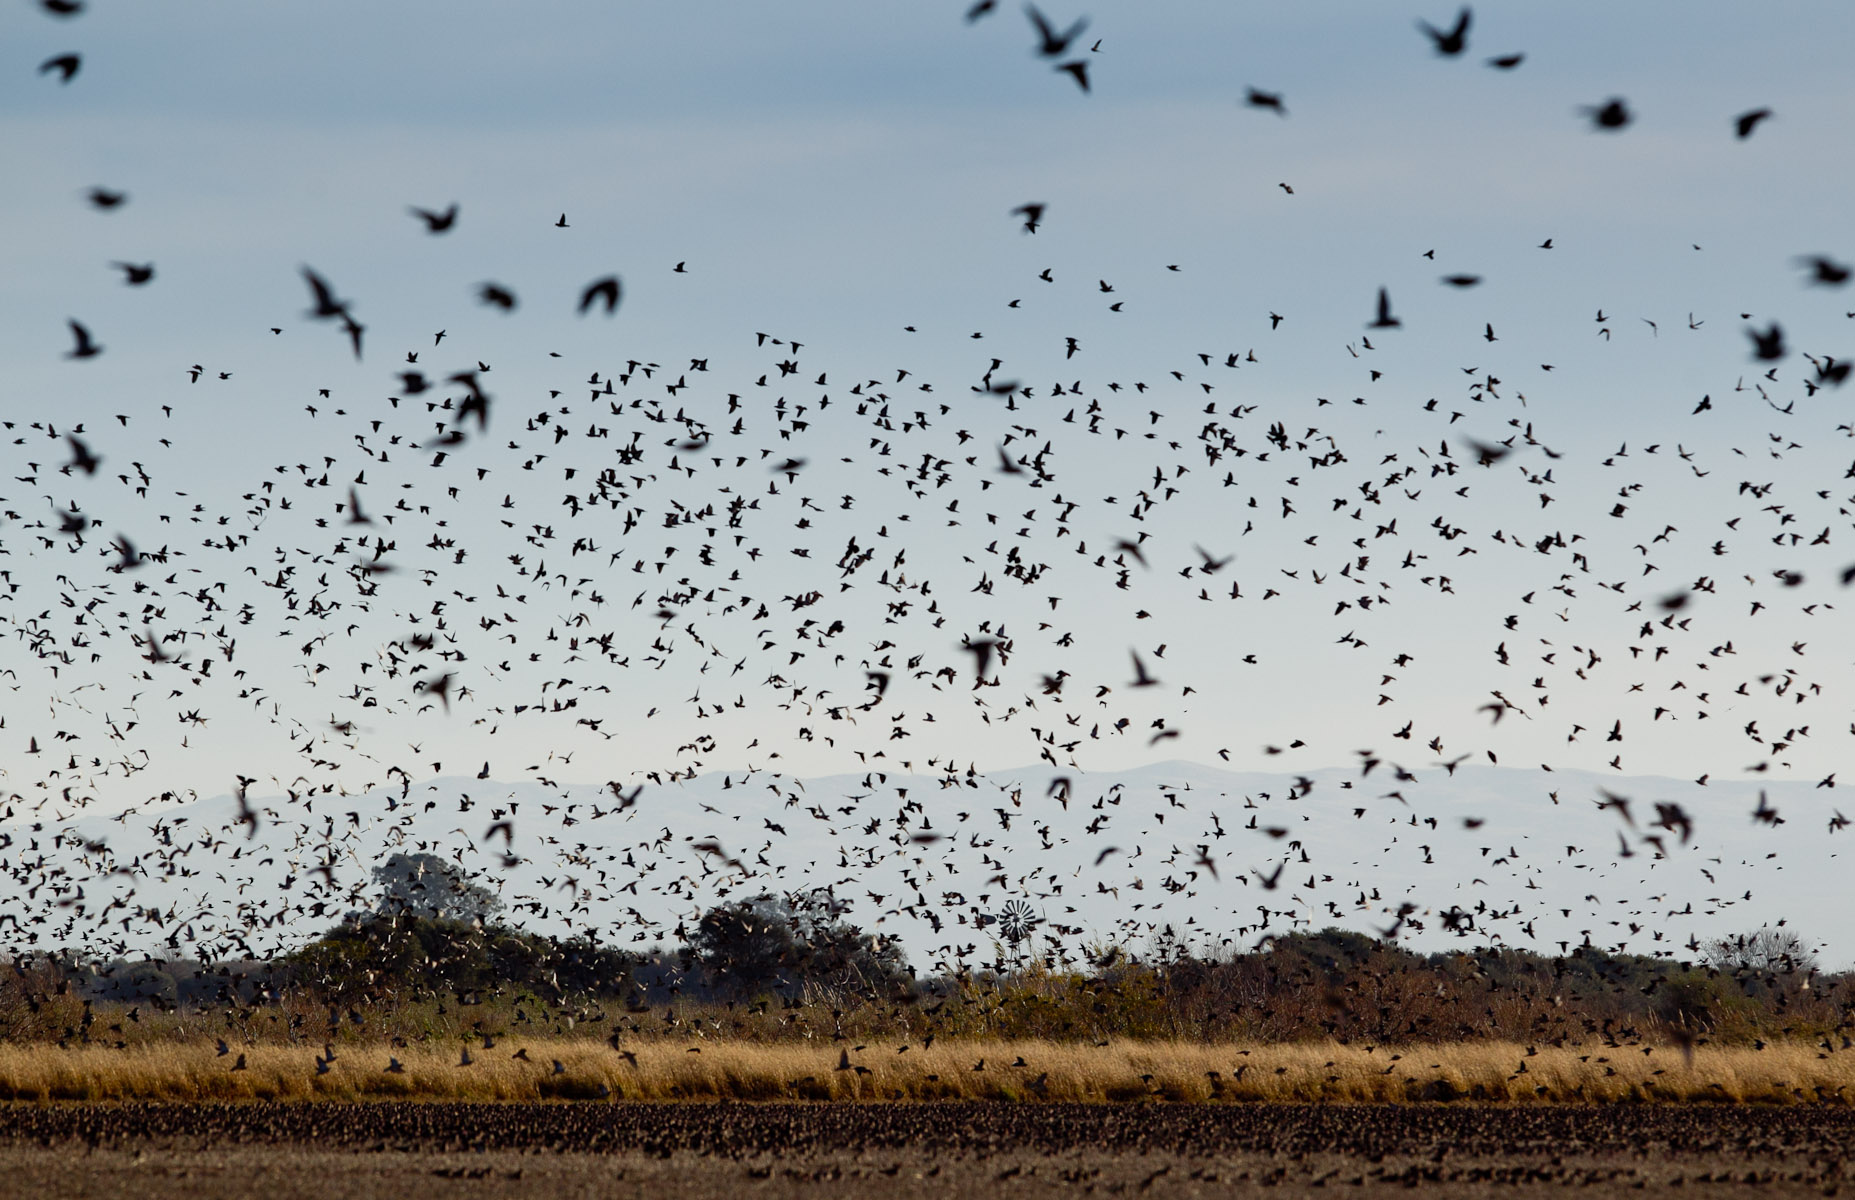
\includegraphics[width=\paperwidth,trim=0mm 0mm 0mm 5.5cm,clip]{figs/doves}
  }
}
\begin{frame}[plain]
  \vspace{-4.2cm}
  \begin{center}
    {\huge Geometric and Exponential Growth } \\
    {\large January 16, 2019 \\}
  \end{center}
  \begin{columns}
    \wide
    \rule[11pt]{\paperwidth}{0.1pt}
  \end{columns}
\end{frame}
}





\section{Background and Review}



\begin{frame}[plain]
  \frametitle{Today's learning objectives}
  \Large
  The equations for geometric and exponential growth \\
  \pause
  \vfill
  The relationship between geometric growth and the BIDE model \\
  \pause
  \vfill
  The difference between continuous and discrete time models
  population growth \\
  \pause
  \vfill
  The definition of density \textit{independent} population growth \\
\end{frame}





% \begin{frame}
%   \frametitle{Outline}
%   \large
%   \only<1>{\tableofcontents[hideallsubsections]}
%   \only<2>{\tableofcontents[currentsection,hideallsubsections]}
% \end{frame}




\begin{frame}
  \frametitle{What is Population Dynamics?}
  {\centering \Large \bf The study of spatial and temporal variation in
    population size and structure \\ }
\end{frame}






\begin{frame}%[t]
  \frametitle{Fundamental Question}
  \begin{center}
   { \Large How does abundance go from $N_t$ to $N_{t+1}$?} \par
   \vspace{1.5cm}
   \large
   \pause
   Answer: The {\color{red} BIDE} Model  \\
     $N_{t+1} = N_t + {\color{red}B}_t + {\color{red}I}_t - {\color{red}D}_t - {\color{red}E}_t$
  \vspace{2mm}
  \end{center}
  B=Births, I=Immigrations, D=Deaths, E=Emigrations \\
  \pause
  \vfill
  Geometric growth is a simplification of BIDE. \\
  \vspace{2mm}
  Exponential growth is a continuous time version of geometric growth.
\end{frame}



%\section{Classical Growth Models}
%\section{From BIDE To Exponential Growth}
\section{Geometric Growth}



% \begin{frame}
%   \frametitle{Outline}
%   \large
%   \tableofcontents[currentsection,hideallsubsections]
% \end{frame}





\begin{frame}
  \frametitle{Reverend Thomas Malthus, 1766--1834}
  \begin{beamercolorbox}[wd=\paperwidth]{white}
    \begin{center}
      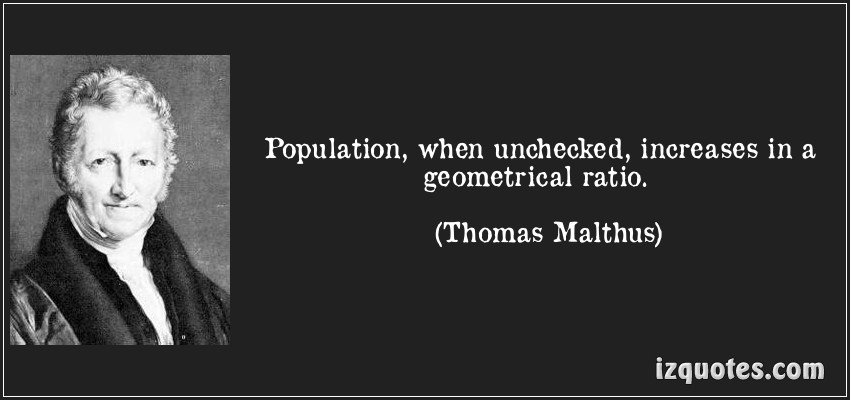
\includegraphics[height=4cm,keepaspectratio]{figs/MalthusGeometric}
      \hspace{0.1cm}
      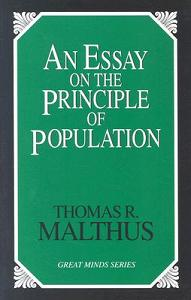
\includegraphics[height=4cm,keepaspectratio]{figs/MalthusBookCover}
    \end{center}
  \end{beamercolorbox}
\end{frame}


\begin{frame}
  \frametitle{\normalsize Relevance To Wildlife Biology and Management}
  Charles Darwin (\textit{Origin of Species})
  \begin{quote}
    ``There is no exception to the rule that every organic being
    increases at so high a rate, that if not destroyed, the earth
    would soon be covered by the progeny of a single pair.''
  \end{quote}
  \pause
  \vfill
  \begin{quote}
    ``Hence, as more individuals are produced than can possibly survive,
    there must in every case be a struggle for existence$\dots$''
  \end{quote}
\end{frame}




\begin{frame}
  \frametitle{\Large Aldo Leopold, Game Management 1946}
  \begin{columns}
    \begin{column}{9cm}
      \small
%      \begin{quote}
      \begin{center}
        \it
        ``Every wild species has certain fixed habits which govern the
        reproductive process, and determine its maximum
        rate. [$\dots$] Thus one pair of quail, if entirely unmolested
        in an ``ideal'' environment, would increase at this rate:''
      \end{center}
%      \end{quote}
      \begin{center}
        \scriptsize
          \begin{tabular}{lrrrr}
            \hline
            At End of && Young & Adults & Total \\
            \hline
            1st year  && 14  & 2   & 16  \\
            2nd year  && (16/2)14=112 & 16  & 128 \\
            3rd year  && (128/2)14=896 & 128 & 1024 \\
            \hline
          \end{tabular}
%        \end{footnotesize}
      \end{center}
      \visible<2>{
%        \begin{quote}
        \begin{center}
          \it
          ``The maximum rate of increase is of course never attained
          in nature. Part of it never takes place, part of it is
          absorbed by natural enemies, and part of it [$\dots$] is
          absorbed by hunters.''
        \end{center}
%        \end{quote}
      }
    \end{column}
%    \hspace{-2cm}
    \begin{column}{2cm}
      \fbox{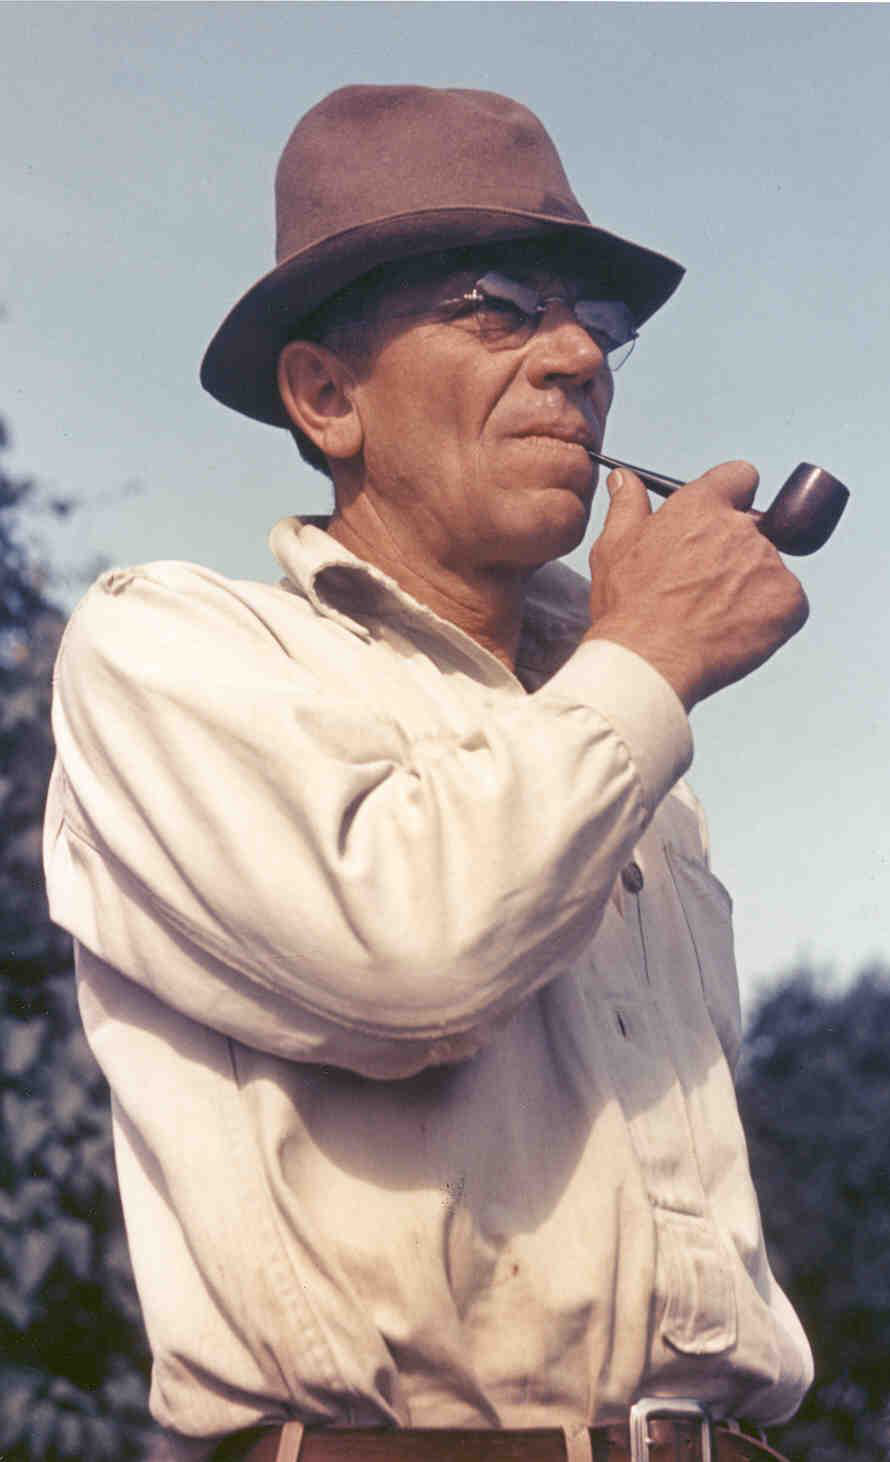
\includegraphics[width=2cm]{figs/Leopold1}} \\ \vspace{0.5cm}
      \fbox{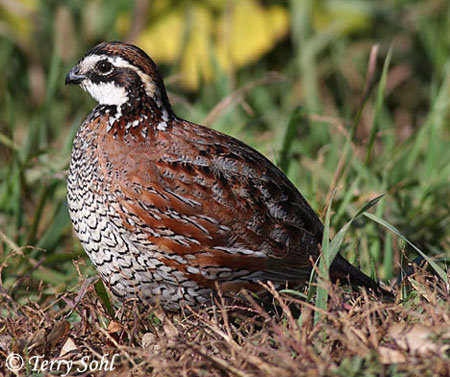
\includegraphics[width=2cm]{figs/nobo}}
    \end{column}
  \end{columns}
\end{frame}






\begin{frame}
  \frametitle{So What Is Geometric Growth?}
    \begin{block}{Discrete time, $t=1,2,\ldots$}
     \begin{center}
       \Large
       $N_t = N_0(1+r)^t$
     \end{center}
     \visible<2>{
     Or, for one time step:
     \begin{center}
       \Large
       $N_{t+1} = N_t + N_tr$
     \end{center}
     }
     $r$ = discrete-time version of intrinsic rate of increase
%     \visible<3>{$\lambda = 1+r$ is the finite rate of increase}
   \end{block}
\end{frame}







\begin{frame}
  \frametitle{Example, $N_{t+1} = N_t + N_tr$}
  \begin{columns}[c]
    \begin{column}{0.5\textwidth}
      \begin{center}
        $N_0 = 3$, $r=1$
        \small
        \begin{tabular}{cc}
          \hline
          Time & Population size \\
          ($t$) & ($N_t$) \\
          \hline
          0 & 3  \\
          \visible<2->{1 & 6}  \\
          \visible<3->{2 & 12} \\
          \visible<4->{3 & 24} \\
          \visible<5->{4 & 48} \\
          \visible<6->{5 & 96} \\
          \visible<7->{6 & 192} \\
          \visible<8->{7 & 384} \\
          \visible<9->{8 & 768} \\
          \visible<10->{9 & 1536} \\
          \visible<11->{10 & 3072} \\
          \hline
        \end{tabular}
      \end{center}
    \end{column}
    \begin{column}{0.5\textwidth}
      \includegraphics<1 | handout:0>[width=\textwidth]{figs/growth0} %\\
      \includegraphics<2 | handout:0>[width=\textwidth]{figs/growth1} %\\
      \includegraphics<3 | handout:0>[width=\textwidth]{figs/growth2} %\\
      \includegraphics<4 | handout:0>[width=\textwidth]{figs/growth3} %\\
      \includegraphics<5 | handout:0>[width=\textwidth]{figs/growth4} %\\
      \includegraphics<6 | handout:0>[width=\textwidth]{figs/growth5} %\\
      \includegraphics<7 | handout:0>[width=\textwidth]{figs/growth6} %\\
      \includegraphics<8 | handout:0>[width=\textwidth]{figs/growth7} %\\
      \includegraphics<9 | handout:0>[width=\textwidth]{figs/growth8} %\\
      \includegraphics<10 | handout:0>[width=\textwidth]{figs/growth9}
      \includegraphics<11>[width=\textwidth]{figs/growth10}
    \end{column}
  \end{columns}
\end{frame}







\begin{frame}
  \frametitle{Three Possible Outcomes, $N_{t+1} = N_t + N_tr$}
  \begin{columns}
    \begin{column}{0.33\textwidth}
      \small
      \centering
      If $-1 \leq r < 0$ \\ population goes extinct \\
      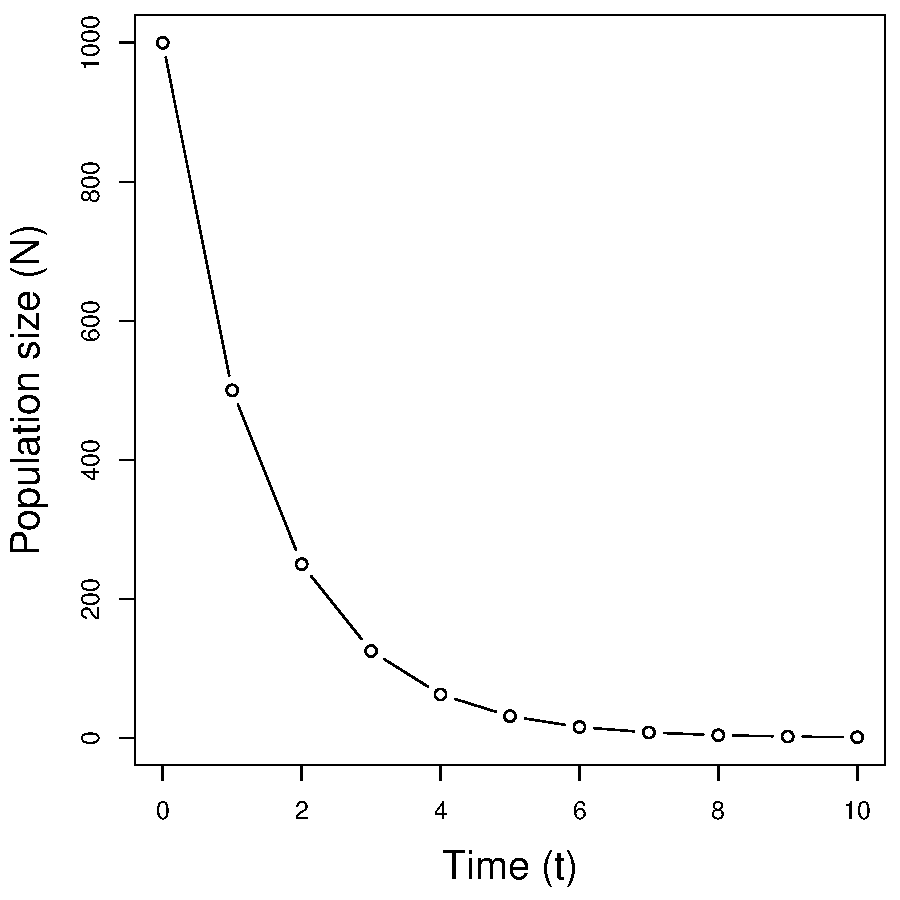
\includegraphics[width=\textwidth]{figs/rl0}
    \end{column}
    \begin{column}{0.33\textwidth}
      \small
      \centering
      If $r = 0$ \\ population is stable \\
      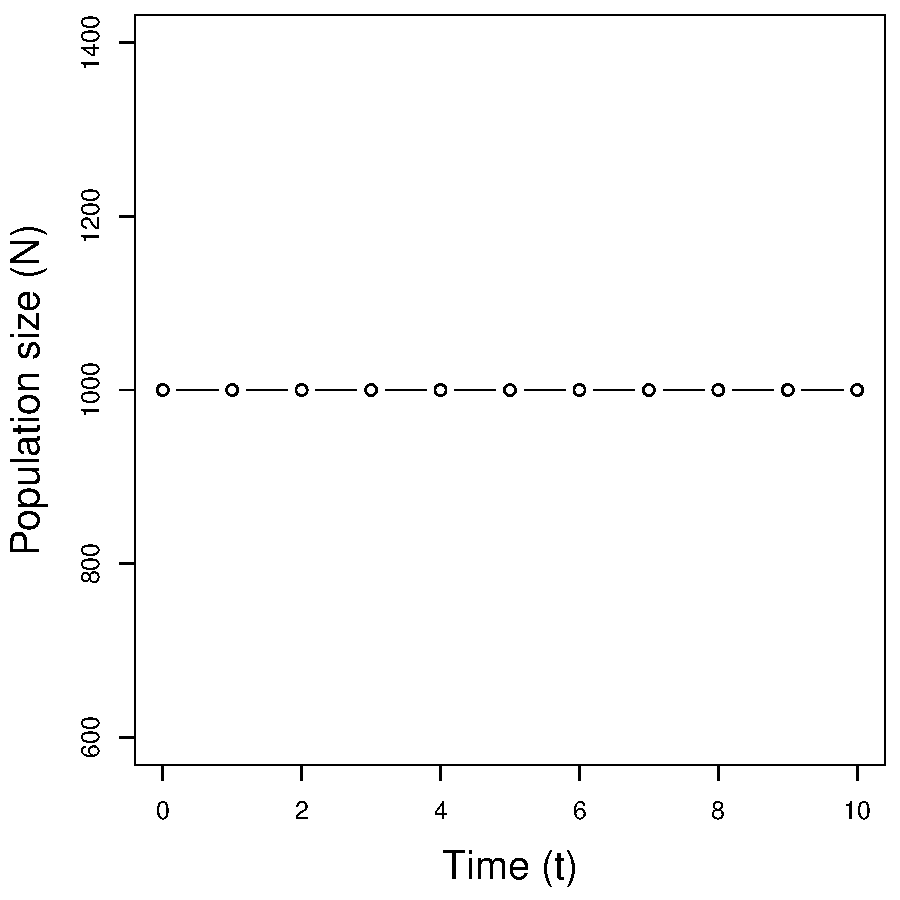
\includegraphics[width=\textwidth]{figs/r0}
    \end{column}
    \begin{column}{0.33\textwidth}
      \small
      \centering
      If $r > 0$ \\ population grows to $\infty$ \\
      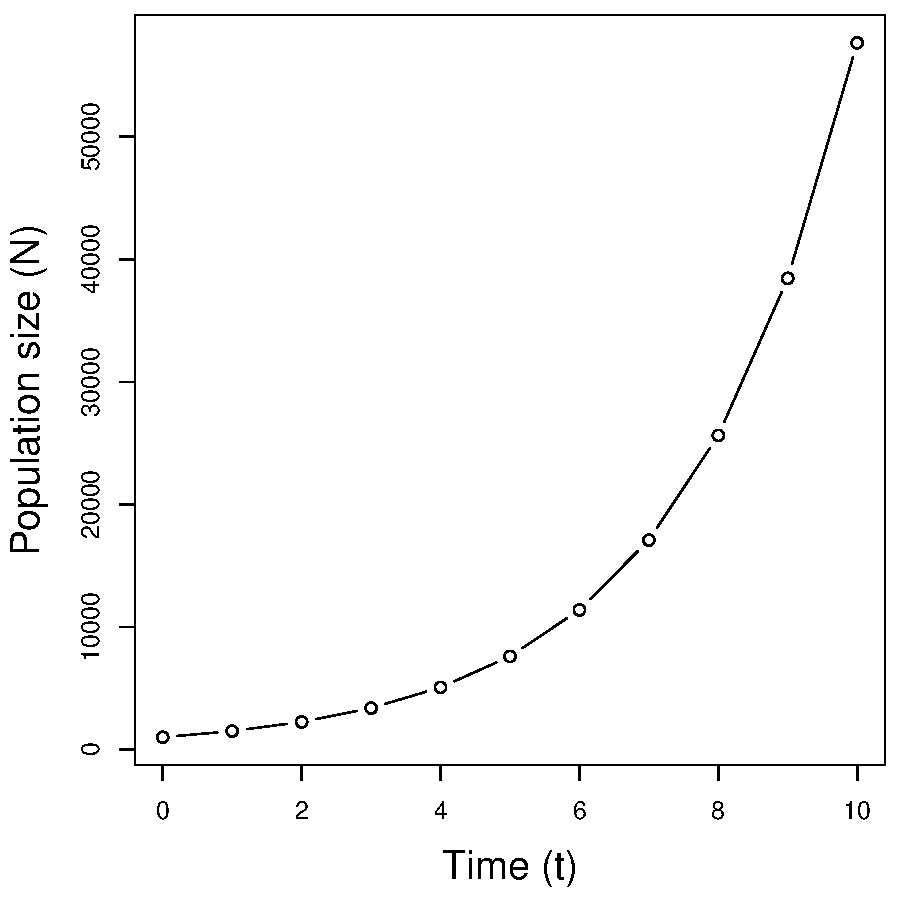
\includegraphics[width=\textwidth]{figs/rg0}
    \end{column}
  \end{columns}
\end{frame}







\begin{frame}
  \frametitle{$r$ and $\lambda$, $N_{t+1} = N_t + N_tr$}
  \Large
%  \bf
  $r$ is the discrete growth rate \par
  \vspace{0.5cm}
  $\lambda$ is the finite growth rate \par
  \[
  \lambda = \frac{N_{t+1}}{N_t}
  \]
%  \pause
  \vspace{0.5cm}
  $\lambda = 1 + r$
\end{frame}





\section{Connection to BIDE}




\begin{frame}
  \frametitle{From {\color{red} BIDE} To Geometric Growth}
%  {\bf \large And how is it related to BIDE model?}
  {\bf \large Fundamental equation of population ecology}
  \[
  N_{t+1} = N_t + B_t + I_t - D_t - E_t
  \]
  \vspace{0.5cm}
  \begin{tabular}{ccl}
    $N_t$ & = & Abundance at year $t$ \\
    {\color{red} $B$}    & = & Births       \\
    {\color{red} $I$}    & = & Immigrations \\
    {\color{red} $D$}    & = & Deaths       \\
    {\color{red} $E$}    & = & Emigrations \\
  \end{tabular}
\end{frame}


\begin{frame}
  \frametitle{From {\color{red} BIDE} To Geometric Growth}
  {\bf \large Ignore immigration and emigration}
  \[
  N_{t+1} = N_t + B_t - D_t
  \]
  \vspace{0.5cm}
  \begin{tabular}{ccl}
    $N_t$ & = & Abundance in year $t$ \\
    {\color{red} $B$}    & = & Births       \\
    {\color{red} $D$}    & = & Deaths       \\
  \end{tabular}
\end{frame}


\begin{frame}
  \frametitle{From {\color{red} BIDE} To Geometric Growth}
    \textbf{Step 1:} Divide both sides by $N_{t}$
      \[
        \frac{N_{t+1}}{N_{t}} \quad = \quad 1 + \frac{B_t}{N_{t}} - \frac{D_t}{N_{t}}
      \]
   \pause
    \textbf{Step 2:} Write in terms of \textit{per capita} birth and death \textit{rates}
      \[
        \frac{N_{t+1}}{N_{t}} \quad  = \quad 1 + b - d \quad = \quad 1 + r \quad = \quad \lambda
      \]
    \pause
    \textbf{Step 3:} Geometric growth \par
    \begin{center}
      $N_{t+1} = N_t + N_tr$
    \end{center}
\end{frame}





% \begin{comment}
%   \begin{frame}
%     \frametitle{What Factors Influence $r$?}
%     \textbf{Minimum age of reproduction}
%     \vspace{.3cm} 
%     \textbf{Young produced per year}
%     \begin{itemize}
%       \item Fertility (e.g. eggs/female)
%       \item Broods per year
%       \item Mating system (monogamous, polygynous, etc...)
%       \item etc\dots
%     \end{itemize}
%     \vspace{.3cm} \textbf{Age structure}
%     \vspace{.3cm} \textbf{Sex ratio}
%     \vspace{.3cm} \textbf{Longevity}
%   \end{frame}
% \end{comment}




%\section{Classical Growth Models}
%\section{From BIDE To Exponential Growth}
\section{Exponential Growth}




%\begin{comment}
\begin{frame}
  \frametitle{So What Is Exponential Growth?}
  \begin{block}{Continuous time version of geometric growth}
    \begin{center}
      \Large
      $N_t = N_0 {e}^{rt}$
    \end{center}
    \visible<2->{
      Or, in terms of instantaneous rate of change:
    \begin{center}
      \Large
      $\frac{\mathrm{d}N}{\mathrm{d}t} = rN$
    \end{center}
    }
    $N_0$ = initial abundance \\
    $r$ = intrinsic rate of increase \\
    $t$ = time (any positive number)
  \end{block}
  \visible<3>{
    \small
    Appropriate if reproduction occurs throughout the year
      (birth flow populations), instead of during short seasons (birth
      pulse populations)
  }
\end{frame}
%\end{comment}




\begin{frame}
  \frametitle{Density Independent Growth}
  \large
  \textbf{Geometric and exponential growth are examples of \alert{\bf
      density independent} growth} \\
  \vspace{0.5cm}
  \pause
  \textbf{Definition:} Population growth rate ($r$) is \textit{not} affected by
    population size ($N$). \\
  \pause
  \vspace{0.5cm}
  \textbf{Implications}:  Resources are unlimited and there is no carrying capacity!
\end{frame}








\begin{frame}
  \frametitle{Model Assumptions}
  \large
  \begin{itemize}
  \item[{\color{beamer@blendedblue} \bf (1)}] {Population is geographically closed}
    \begin{itemize}
      \large
      \item No immigration
      \item No emigration
    \end{itemize}
    \visible<2->{
      \vfill
    \item[{\color{beamer@blendedblue}\bf (2)}] {Reproduction
        occurs seasonally (for geometric growth)}
%      \begin{itemize}
%        \large
%        \item Reproduction occurs seasonally
%      \end{itemize}
    }
    \visible<3->{
      \vfill
    \item[{\color{beamer@blendedblue}\bf (3)}] {Constant birth rate ($b$) and death rate ($d$)}
      \begin{itemize}
        \large
        \item No genetic variation among individuals
        \item No age- or stage-structure
        \item No time lags
      \end{itemize}
    }
    \visible<4>{
      \vfill
    \item[{\color{beamer@blendedblue}\bf (4)}] {No stochasticity}
      \begin{itemize}
        \large
        \item No random variation in birth or death 
        \item No random variation in environmental conditions
      \end{itemize}
    }
  \end{itemize}
\end{frame}



% \begin{frame}
%   \frametitle{Extensions}
%   \textbf{Growth rate is usually not constant}
%   \vspace{0.8cm}
%   \begin{columns}
%     \begin{column}{0.5\textwidth}
% %      \textbf{Growth rate is usually not constant}
% %      \begin{itemize}
%         $r$ might depend on habitat \\ \vspace{2cm}
%         Or, chance (stochasticity) might play a role
% %      \end{itemize}
%     \end{column}
%     \begin{column}[c]{0.5\textwidth}
%       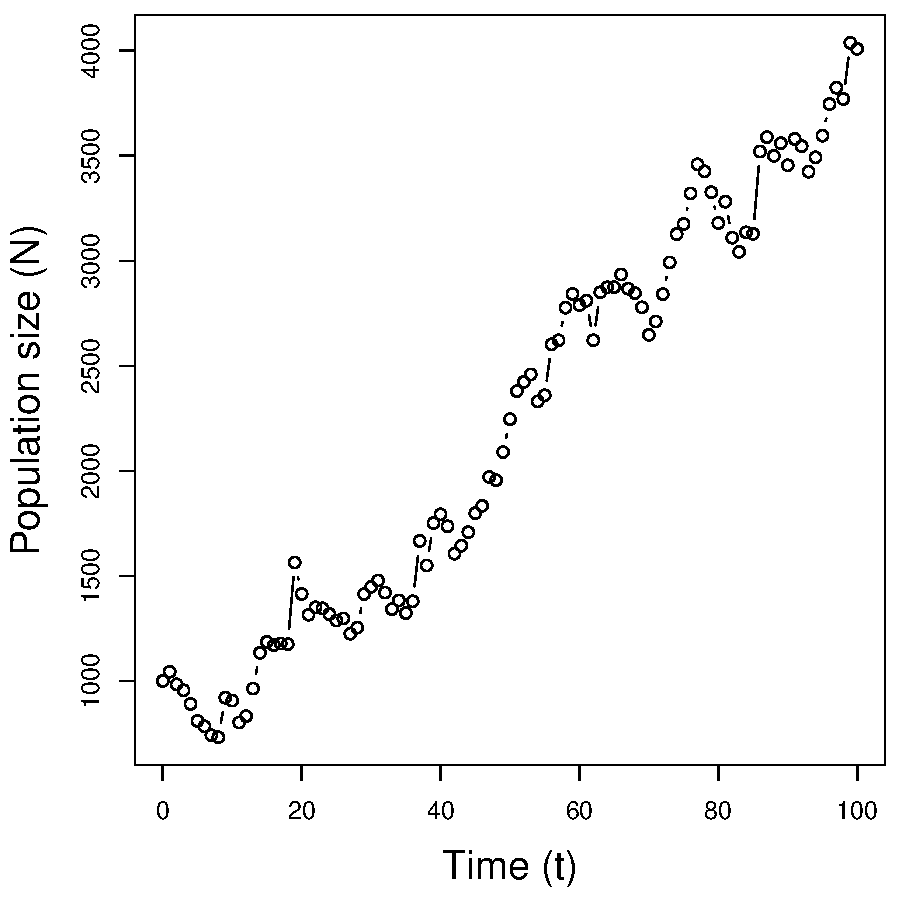
\includegraphics[width=\textwidth]{figs/rg0st}
%     \end{column}
%   \end{columns}
% \end{frame}





\begin{frame}
%  \frametitle{Of What Use is This?}
  \frametitle{\large Can We Apply The Model To Real Data?}
  {All models are wrong, but some are useful. (George Box)} \\ 
  \vspace{0.5cm}
  \visible<2->{
  {Is exponential growth a useful model?}
  }
  \visible<3->{
  \begin{itemize}
  \item Possibly for describing some populations during short time
    periods, e.g. invasive species or prey following removal of
    predators
  \item Also useful as foundation for more realistic models
  \end{itemize}
  \begin{center}
    \fbox{
      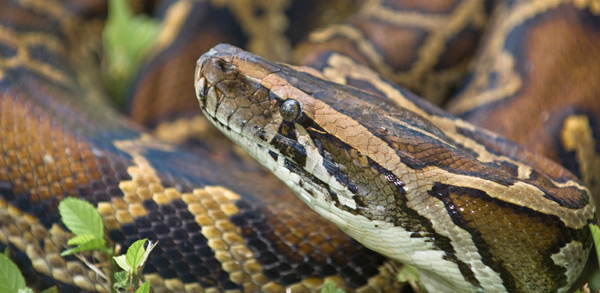
\includegraphics[height=2.5cm,keepaspectratio]{figs/python1} \hspace{0.1cm}
      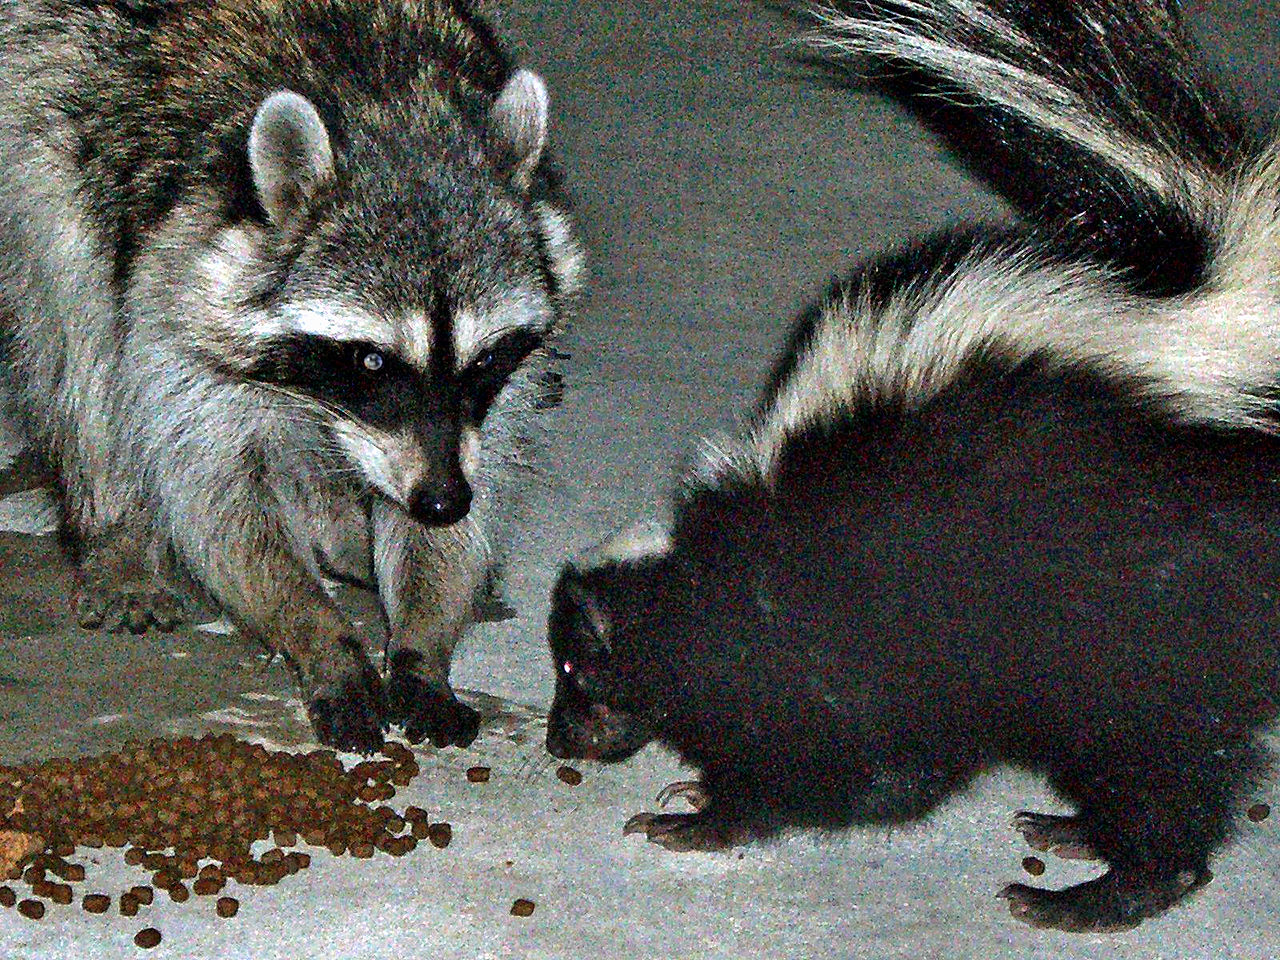
\includegraphics[height=2.5cm,keepaspectratio]{figs/racoon_skunk}
    }
  \end{center}
  }
\end{frame}





% \begin{frame}
%   \frametitle{\large Can We Apply The Model To Real Data?}%Is This A Good Model?}
%   \begin{center}
%     \only<1 | handout:0>{\includegraphics[width=.8\textheight]{figs/MalthusVdata1}}
%     \only<2>{\includegraphics[width=.8\textheight]{figs/MalthusVdata2}}
% %    \only<3>{\includegraphics[width=.8\textheight]{figs/MalthusVdata3}}
%   \end{center}
% \end{frame}









% \begin{frame}
%   \frametitle{Recap}
%   {\bf For one time step, geometric growth is:\par}
%   {\large \centering $N_{t+1} = N_t + N_tr$ \par}
%   \vspace{0.5cm}
%   {\bf For arbitrary time steps, geometric growth is:\par}
%   {\large \centering $N_{t} = N_{0}(1+r)^t$ \par}
%   \vspace{0.5cm}
%   {\bf Definitions: \par}
%     \begin{itemize}
%       \item $r = b-d$ is discrete growth rate
%       \item $b = B/N$ is per capita birth rate (births/individual)
%       \item $d = D/N$ is per capita death rate (probability of dying)
%     \end{itemize}
% \end{frame}







\begin{frame}
  \frametitle{Looking Ahead}
  \begin{center}
    {\large \bf Density dependence and logistic growth}
    \includegraphics[width=0.6\textwidth]{figs/UN-population}
  \end{center}
\end{frame}


%\renewcommand*{\refname}{}
%\begin{frame}
%  \frametitle{References}
%  \bibliography{popdyn}
%\end{frame}




\begin{frame}
  \frametitle{Assignment}
  \Large
  Read pages 15--19 in Conroy and Carroll \\
  \vspace{1cm}
  Be prepared for a quiz \\
\end{frame}




\end{document}






































% \section{Applications to Management}



% \begin{frame}
%   \frametitle{Outline}
%   \large
%   \tableofcontents[currentsection,hideallsubsections]
% \end{frame}







% %\subsection{Game Species}


% %``We Americans, in most states at least, have not yet experienced a
% %bear-less, eagle-less, cat- less, wolf-less woods. Germany strove for
% %maximum yields of both timber and game and got neither.'' Notes on Wild
% %Life Conservation in Germany (1935) LP: Writings: Reprints (bound):
% %Publications of Aldo Leopold: game 735

% \begin{frame}[t]
%   \frametitle{Setting Harvest Limits}
%   \textbf{How many individuals can be harvested to maintain a stable
%     population?} \par
%   \only<1>{
%   \begin{center}
% %    \setlength\fboxsep{0pt}
%     \fbox{\only<1>{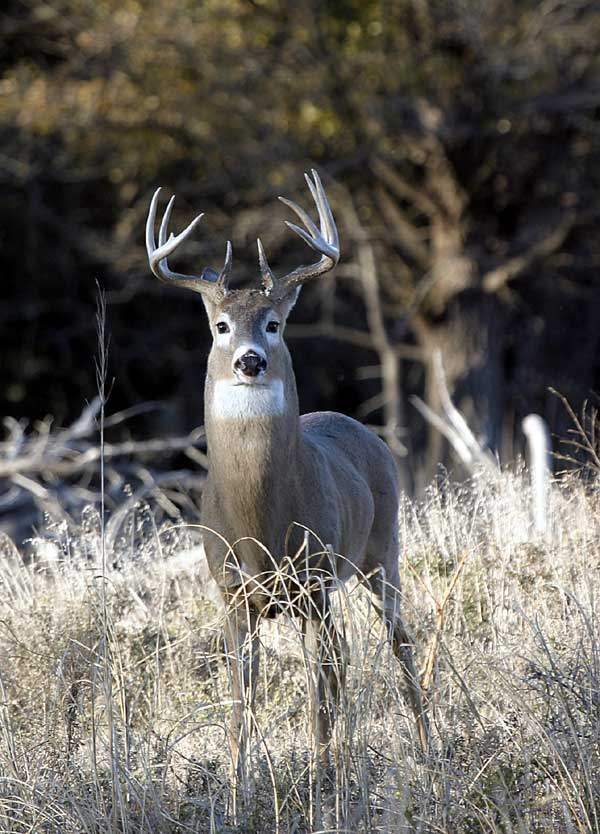
\includegraphics[height=0.7\textheight]{figs/buck1}}}
%   \end{center}
%   }
% %  \only<2->{
%   \vspace{0.2cm}
%   \visible<2->{
%   \textbf{Step 1:} Change the model to this:

%   \begin{center} $N_{t+1} = N_t + N_tr - H$ \end{center}

%   \hspace{1.5cm} where $H$ is the number of harvested animals.
%   }

%   \vspace{0.8cm}
%   \visible<3->{
%   {\bf Step 2:} Set $N_{t+1} = N_t$ and solve for $H$:

%   \begin{center} $H = N_tr$ \end{center}
%   }

%   \vspace{0.1cm}
%   \visible<4>{
%   \textbf{So, we want to remove $H = N_tr$ animals from the
%     population} \par
%   }
% %  }
% \end{frame}








%\subsection{Declining Species}



%\begin{frame}
%  \frametitle{Additive vs. Compensatory Mortality}
%\end{frame}


% \begin{frame}
%   \frametitle{Time to Extinction}
%   {\large \bf In what year will the population fall below, say, $N=10$?}
%    \begin{center}
%      \includegraphics<1>[width=0.8\textwidth]{figs/decline1}
%      \includegraphics<2>[width=0.8\textwidth]{figs/decline2}
%      \includegraphics<3>[width=0.8\textwidth]{figs/decline3}
%    \end{center}
% \end{frame}


\begin{comment}
\section{Bear Example}


\begin{frame}
  \frametitle{Outline}
  \large
  \tableofcontents[currentsection,hideallsubsections]
\end{frame}


%\subsection{Bear Example}

\begin{frame}
  \frametitle{Louisiana Black Bear}
%  \vspace{-0.4cm}
  \begin{center}
    \textit{Ursus americanus luteolus} %\\
    \fbox{
    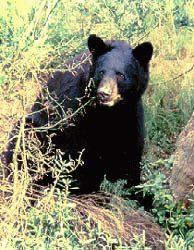
\includegraphics[height=0.6\textheight,keepaspectratio]{figs/LAbear1} \hspace{0.2cm}
    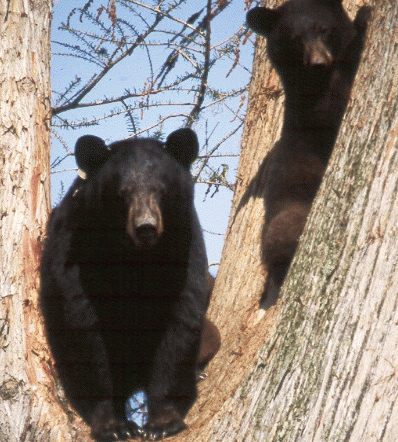
\includegraphics[height=0.6\textheight,keepaspectratio]{figs/LAbear2}
    }
  \end{center}
\end{frame}


\begin{frame}
  \frametitle{Louisiana Black Bear}
%  \vspace{-0.4cm}
  \begin{center}
    \setlength\fboxsep{0pt}
    \fbox{
    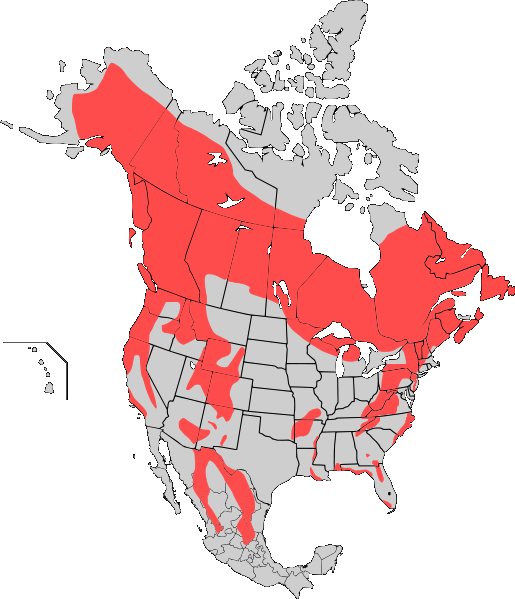
\includegraphics[height=0.6\textheight,keepaspectratio]{figs/Black_bear_map} \hspace{0.2cm}
    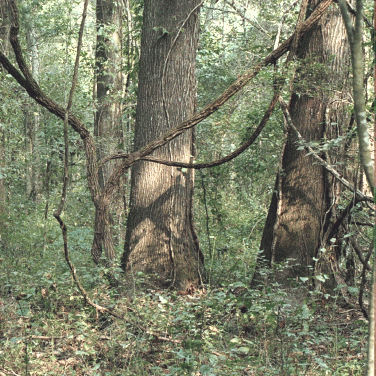
\includegraphics[height=0.6\textheight,keepaspectratio]{figs/LAbearHabitat1}}
  \end{center}
\end{frame}


\begin{frame}
  \frametitle{Louisiana Black Bear}
  \large
%  \begin{itemize}
    \textbf{1 of 16 recognized subspecies} \\ \vspace{0.5cm}
    \textbf{Federally listed threatened subspecies}\\ \vspace{0.5cm}
    \textbf{Threats include:}
      \begin{itemize}
        \item genetic isolation from habitat fragmentation
        \item habitat loss
        \item poaching
        \item vehicle collisions
      \end{itemize}
%  \end{itemize}

\end{frame}


\begin{frame}
  \frametitle{Study Design}
  \begin{columns}
    \begin{column}{0.5\textwidth}
      \large
      \textbf{3 years of data collection (2007-2009)} \\
      \vspace{0.5cm}
      \textbf{115 baited hair snares} \\
      \vspace{0.5cm}
      \textbf{Capture-recapture methods used to estimate $N_t$ and $r$}
    \end{column}
    \begin{column}{0.3\textwidth}
      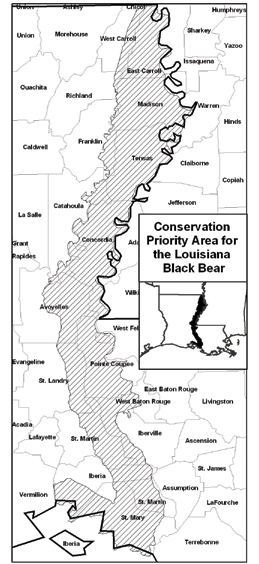
\includegraphics[width=\textwidth]{figs/bearMap1}
    \end{column}
  \end{columns}
\end{frame}




\begin{frame}
  \frametitle{Exponential Model Results}
  \begin{center}
%    \Large
    \begin{tabular}{llr}
      \hline
      Parameter & Description                        & Estimate \\
      \hline
      $b$       & Female cubs born per adult female  & 0.687    \\
      $d$       & Mortality rate                     & 0.178    \\
      $r$     & Growth rate                        & 0.509    \\
      \hline
    \end{tabular}
  \end{center}
  \visible<2->{\textbf{Is the population growing or declining?}} \\
  \vspace{0.5cm}
  \visible<3>{\textbf{Growing because $r>0$}}
\end{frame}




\begin{frame}
  \frametitle{Exponential Model Results}
  \begin{center}
    \only<1>{\includegraphics[width=0.9\textwidth]{figs/bearNF1}}
    \only<2>{\includegraphics[width=0.9\textwidth]{figs/bearNF2}}
  \end{center}
%  \visible<2>{\textbf{Not a good model!}}
\end{frame}



\begin{frame}
  \frametitle{Implications}
  \begin{quote}
%    \large
    ``LDWF has made delisting the Louisiana black bear one of its
    highest priorities. Transforming a perceived nuisance animal to a
    trophy game animal will be one of the greatest endangered species
    success stories to occur in Louisiana.'' \\
    \vspace{0.5cm}
    \small
    --Louisiana Department of Wildlife and Fisheries, 2010
  \end{quote}
\end{frame}



\begin{frame}
  \frametitle{What Would Be Optimal Harvest?}
  \visible<2->{{\color{red} \bf Don't harvest threatened (sub)species!} \\}
  \vspace{0.5cm}
  \visible<3->{\textbf{But, for argument's sake, what would be the optimal harvest
    size ($H$) to maintain a population of $N=100$ bears?}} \\
  \vspace{0.5cm}
  \visible<4->{\textbf{Answer:} $H = Nr = 100\times0.509 = 50.9 \text{bears}$}
\end{frame}





\begin{frame}
  \frametitle{Real World}
  \textbf{Populations typically don't grow exponentially} \\
  \vspace{0.5cm}
  \visible<2->{
  \textbf{We don't know $r$ or $N_t$} \\
  }
  \vspace{0.5cm}
  \visible<3->{
  \textbf{$r$ changes unpredictably} \\
  }
  \vspace{0.5cm}
  \visible<4->{
  \textbf{Conclusion:} Managing populations is very difficult, and we
  need a more realistic model.
  }
\end{frame}




\end{comment}


